\documentclass[conference]{sty/IEEEtran}
\usepackage{times}
\usepackage{wrapfig}
\usepackage{tweaklist}
\usepackage{xspace}
\usepackage{graphicx}
\usepackage{subfigure}
\usepackage{tabularx}
\usepackage{amsmath}
\usepackage{amssymb}
\usepackage{url}


% numbers option provides compact numerical references in the text. 
\usepackage[numbers]{natbib}
\usepackage{multicol}
\usepackage[bookmarks=true]{hyperref}

\pdfinfo{
   /Author (Homer Simpson)
   /Title  (Robots: Our new overlords)
   /CreationDate (D:20101201120000)
   /Subject (Robots)
   /Keywords (Robots;Overlords)
}

\begin{document}

% paper title
%\title{Classification of Objects of Daily Use Using Combined Color CHLAC and Global Radius-based Surface Descriptors}
\title{Multidimensional Descriptor for Classification of Objects of Daily Use}

% You will get a Paper-ID when submitting a pdf file to the conference system
\author{Author Names Omitted for Anonymous Review. Paper-ID [add your ID here]}

%\author{\authorblockN{Michael Shell}
%\authorblockA{School of Electrical and\\Computer Engineering\\
%Georgia Institute of Technology\\
%Atlanta, Georgia 30332--0250\\
%Email: mshell@ece.gatech.edu}
%\and
%\authorblockN{Homer Simpson}
%\authorblockA{Twentieth Century Fox\\
%Springfield, USA\\
%Email: homer@thesimpsons.com}
%\and
%\authorblockN{James Kirk\\ and Montgomery Scott}
%\authorblockA{Starfleet Academy\\
%San Francisco, California 96678-2391\\
%Telephone: (800) 555--1212\\
%Fax: (888) 555--1212}}


% avoiding spaces at the end of the author lines is not a problem with
% conference papers because we don't use \thanks or \IEEEmembership


% for over three affiliations, or if they all won't fit within the width
% of the page, use this alternative format:
% 
%\author{\authorblockN{Michael Shell\authorrefmark{1},
%Homer Simpson\authorrefmark{2},
%James Kirk\authorrefmark{3}, 
%Montgomery Scott\authorrefmark{3} and
%Eldon Tyrell\authorrefmark{4}}
%\authorblockA{\authorrefmark{1}School of Electrical and Computer Engineering\\
%Georgia Institute of Technology,
%Atlanta, Georgia 30332--0250\\ Email: mshell@ece.gatech.edu}
%\authorblockA{\authorrefmark{2}Twentieth Century Fox, Springfield, USA\\
%Email: homer@thesimpsons.com}
%\authorblockA{\authorrefmark{3}Starfleet Academy, San Francisco, California 96678-2391\\
%Telephone: (800) 555--1212, Fax: (888) 555--1212}
%\authorblockA{\authorrefmark{4}Tyrell Inc., 123 Replicant Street, Los Angeles, California 90210--4321}}


\maketitle

\begin{abstract}
The abstract goes here.
\end{abstract}

\IEEEpeerreviewmaketitle

\section{Introduction}
One of the great challenges faced by autonomous mobile robot
manipulation is the scaling of the technology to realistic tasks, in
realistic environments under realistic conditions. This challenge
implies that an autonomous household robot is required to act on many
different objects of daily use, to handle them in typical situations
for example when opening a fridge to get the milk or when performing
realistic tasks such as setting the table or preparing a meal.

\subsection{What}
Problem statement:
\begin{itemize}
\item Recogniton and localization of objects of daily use in households
\item Categorization and classification with \emph{one} descriptor
\item Omits a supporting-table assumption and performs in cluttered and occluded scenes
\item Runs online
\end{itemize}


\subsection{Why}
\begin{itemize}
\item to equipp the service robots with the boostrapped recognition models and capabilities
to acquire additional models
\item to enable manipulation tasks in realistic environments under realistic conditions
\item to exploit new sensing technology (e.g. Kinect) and to thus avoid decoupling of gemetrical and
visual appearance data
\end{itemize}


\subsection{How}
\begin{itemize}
\item Combination of view-variant ColorCHLAC and GRSD with the
normalization of the latter by number 27 (number of transitions)
\item Combination of view-invariant version of ColorCHLAC and GRSD
\item Comparisson of Linear Subspace Method and SVM Classifier
\end{itemize}

\subsection{Novelty}


\section{Related Work}
\begin{itemize}
\item VFH
\item GRSD (Humanoids10GRSD)\cite{kalman1960new} 
\item Color CHLAC (Asako)
\end{itemize}

\section{System Overview}


\section{Feature Estimation}

\subsection{Color CHLAC}
\subsection{GRSD}
\begin{figure}[htb!]
  \begin{center}
    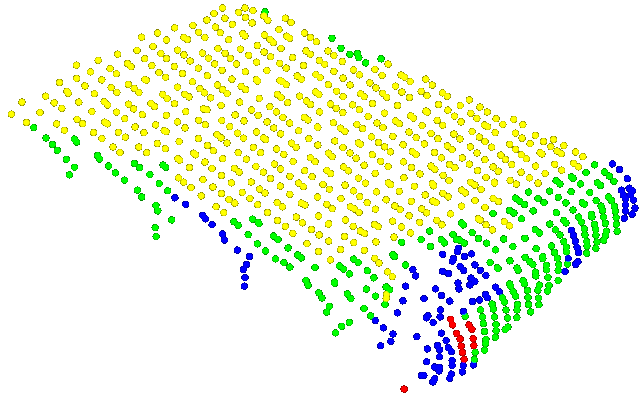
\includegraphics[width=.4\columnwidth]{figures/grsd/book.png}
\hfill
    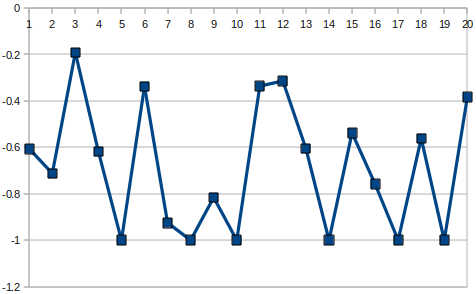
\includegraphics[width=.48\columnwidth]{figures/grsd/book_global.png} \\
\hfill
    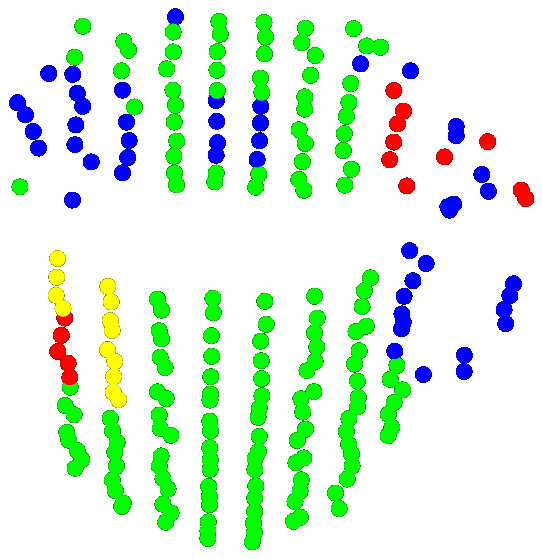
\includegraphics[width=.3\columnwidth]{figures/grsd/mug.png}
\hfill
    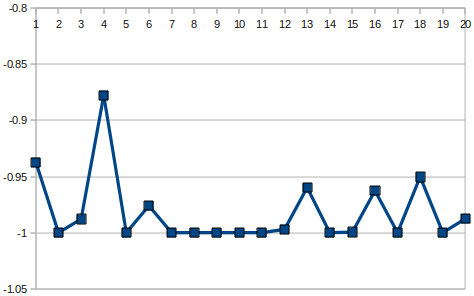
\includegraphics[width=.48\columnwidth]{figures/grsd/mug_global.png}
\caption{Example of RSD classes and GRSD plots for a big flat box (i.e. book, upper row) and a short cylinder (i.e. mug, bottom row).
The histogram bin values are scaled between -1 and 1 according to the
training data, and the colors represent the following local surfaces:
red - sharp edge (or noise), yellow - plane, green - cylinder, light blue -
sphere (not present), and dark blue - rim (i.e. boundary, transition between surfaces).
\emph{Best viewed in color.}
}
    \label{fig:gfpfh}
  \end{center}
\vspace{-2ex}
\end{figure}

\section{Classification Methods}

\subsection{Linear Subspace Method}
\subsection{Support Vector Machine-based Classification}


\section{Results}

\subsection{Data Acquisition and Training}
\begin{figure}[htb!]
  \begin{center}
    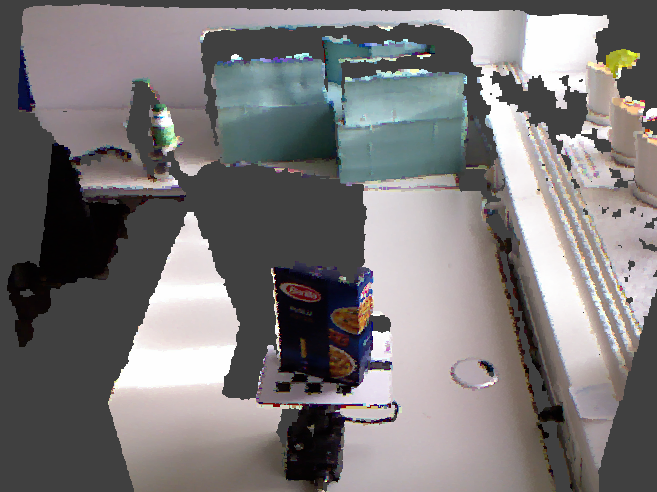
\includegraphics[width=.45\columnwidth]{figures/rot_table/barilla.png}
\hfill
    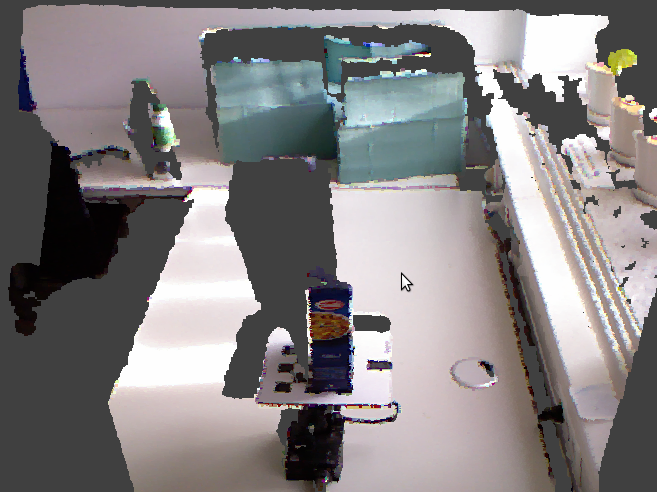
\includegraphics[width=.45\columnwidth]{figures/rot_table/barilla1.png} \\
    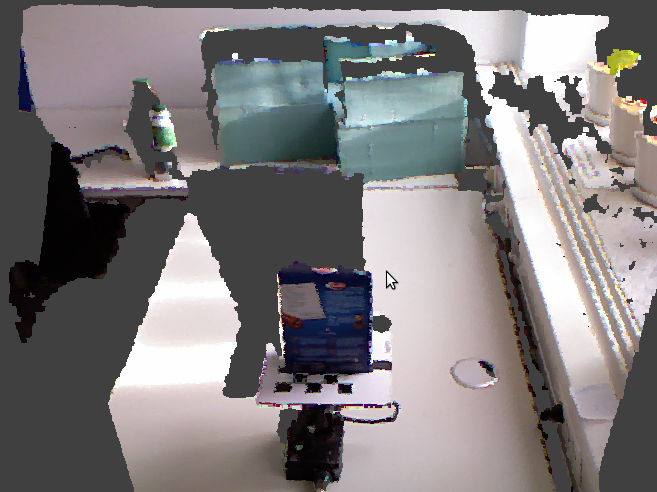
\includegraphics[width=.45\columnwidth]{figures/rot_table/barilla2.png}
\caption{Acquisition of Training Data}
    \label{fig:data_acquisition}
  \end{center}
\end{figure}
\subsection{Online Testing/Object Recognition}

\begin{figure}[htb!]
  \begin{center}
    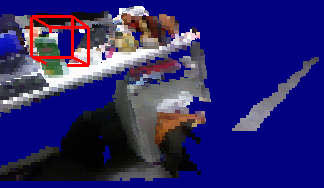
\includegraphics[width=.45\columnwidth]{figures/colorCHLAC/detection7.png}
\hfill
    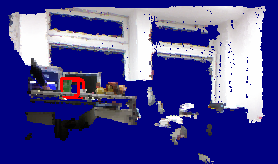
\includegraphics[width=.45\columnwidth]{figures/colorCHLAC/detection5.png} \\
\hfill
    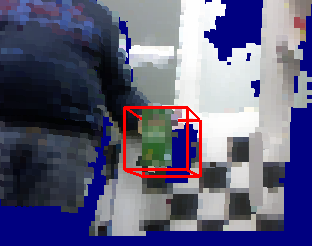
\includegraphics[width=.9\columnwidth]{figures/colorCHLAC/detection2.png}
\caption{An example of the detection of tetrahedral package of milk}
    \label{fig:milk_testing}
  \end{center}
\end{figure}


\section{Conclusions and Future Work} 
The conclusion goes here.

\section*{Acknowledgments}
CoTeSys
%% Use plainnat to work nicely with natbib. 

\bibliographystyle{plainnat}
\bibliography{references}

\end{document}


%TODO:
%Check the original template and see what the meant with the hyperlinks
